\documentclass[10pt,journal]{IEEEtran}
\usepackage{cite}
\usepackage{amsmath,amssymb,amsfonts}
\usepackage{algorithmic}
\usepackage{booktabs}
\usepackage{graphicx}
\usepackage{textcomp}
\usepackage{xcolor}
\usepackage{tikz}
\usetikzlibrary{arrows.meta,positioning,shapes,shapes.geometric,calc,decorations.pathreplacing}
\usepackage{pgfplots}
\pgfplotsset{compat=1.18}
\usepackage{hyperref}
\hypersetup{colorlinks=true,linkcolor=black,citecolor=black,urlcolor=blue}
\def\BibTeX{{\rm B\kern-.05em{\sc i\kern-.025em b}\kern-.08em
    T\kern-.1667em\lower.7ex\hbox{E}\kern-.125emX}}

\begin{document}

\title{AI-Based Web Application to Analyse Genetic Mutations and Disease Impact}


\author{
\begin{tabular}{cc}

% ---------------- ROW 1 ----------------
\begin{tabular}{c}
\IEEEauthorblockN{Vishwaradhya A C\IEEEauthorrefmark{1}}\\
\IEEEauthorblockA{
\textit{Department of Computer Science and Engineering}\\
\textit{College Name, University}\\
author.one@college.edu}
\end{tabular}
&
\begin{tabular}{c}
\IEEEauthorblockN{Nandish S Shet\IEEEauthorrefmark{1}}\\
\IEEEauthorblockA{
\textit{Department of Computer Science and Engineering}\\
\textit{College Name, University}\\
author.two@college.edu}
\end{tabular}
\\[2em]

% ---------------- ROW 2 ----------------
\begin{tabular}{c}
\IEEEauthorblockN{Jeevan A M\IEEEauthorrefmark{1}}\\
\IEEEauthorblockA{
\textit{Department of Computer Science and Engineering}\\
\textit{College Name, University}\\
author.three@college.edu}
\end{tabular}
&
\begin{tabular}{c}
\IEEEauthorblockN{Thippeswamy S\IEEEauthorrefmark{1}}\\
\IEEEauthorblockA{
\textit{Department of Computer Science and Engineering}\\
\textit{College Name, University}\\
author.four@college.edu}
\end{tabular}
\\[2em]

% ---------------- GUIDE ----------------
\multicolumn{2}{c}{
\begin{tabular}{c}
\IEEEauthorblockN{Guide Name\IEEEauthorrefmark{2}~(Faculty Guide)}\\
\IEEEauthorblockA{
\textit{Department of Computer Science and Engineering}\\
\textit{College Name, University}\\
guide.name@college.edu}
\end{tabular}
}

\end{tabular}

\IEEEauthorblockA{
\IEEEauthorrefmark{1}Student\\
\IEEEauthorrefmark{2}Faculty Guide
}
}



\maketitle

\begin{abstract}
Variant interpretation remains a bottleneck in genomic medicine. A single nucleotide change in a gene such as \textit{BRCA1} can be harmless, or it can sharply raise disease risk, and telling the two apart still needs both statistical evidence and biological context. In this work we designed, built and deployed a full-stack web application that brings a large genomic language model directly to this task. The system couples a Next.js front end for genome browsing with a serverless GPU back end that runs the Evo2 model for zero-shot variant scoring. Users pick a human assembly, browse chromosomes or search genes, inspect the reference sequence and known ClinVar entries, and request an Evo2-based pathogenicity call for any single nucleotide variant. Scoring uses an 8192-bp window around the variant, compares reference and alternate sequence likelihoods, and maps the resulting delta score to a calibrated prediction with a confidence estimate derived from a BRCA1 study. On a 500-variant BRCA1 set we observed clear separation between loss-of-function and functional variants with an AUROC around 0.73, consistent with published zero-shot results. The contribution is practical: an accessible, reproducible pipeline from public genome APIs to GPU inference, evaluated on real data with honest discussion of its limits.
\end{abstract}

\begin{IEEEkeywords}
Variant effect prediction, Evo2, genomic language model, BRCA1, ClinVar, Next.js, Modal, UCSC Genome Browser, zero-shot scoring.
\end{IEEEkeywords}

\section{Introduction}
\IEEEPARstart{D}{NA} reads like a very long string over four letters: A, C, G and T. Most positions do not matter much on their own. A few do. When a patient carries an A where the reference has a G inside a cancer-protective gene, the clinical question is immediate: is this change likely benign, or should it change care?

Traditional answers come from population frequency, family studies and curated rules such as the ACMG guidelines~\cite{richards2015acmg}. Those rules work, but they are slow to extend to rare or unseen variants. Computational predictors such as SIFT~\cite{ng2003sift}, PolyPhen-2~\cite{adzhubei2010polyphen} and CADD~\cite{kircher2014cadd} helped by scoring amino-acid or conservation features. More recently protein language models~\cite{lin2023esm,cheng2023alphamissense} and DNA language models~\cite{dalla2023nucleotide,nguyen2024evo,brixi2025evo2} showed that a model trained only to predict the next token can already capture a surprising amount of biological constraint.

We wanted to make that capability usable outside a notebook. This paper describes what we actually built: a web application where a user can start from ``which assembly?'' and end with ``what does Evo2 think of this variant, and how does that compare with ClinVar?'' The front end handles genome navigation and data gathering, the back end handles GPU inference, and a small calibration layer turns raw likelihoods into a readable call with confidence.

Our contributions are:
\begin{itemize}
\item An end-to-end architecture joining UCSC~\cite{kent2002ucsc,lee2022ucsc}, NCBI E-utilities/ClinVar~\cite{landrum2014clinvar,landrum2023clinvar}, a Modal H100 service and a Next.js interface.
\item A concrete scoring procedure based on Evo2~\cite{brixi2025evo2}: 8192-bp windowing, reference-vs-alternate likelihood comparison, ROC-based thresholding with Youden's index~\cite{youden1950index} and class-conditional confidence.
\item An evaluation on 500 \textit{BRCA1} single nucleotide variants with distribution and ROC analysis, plus a live single-variant path demonstrated on \textit{BRCA1} chr17.
\item A candid account of limits: SNV-only support, hg19-derived thresholds applied to hg38 queries, and caps in public API usage.
\end{itemize}

\section{Background: What the Model Actually Sees}
A reader without a biology background needs only four ideas. First, DNA is double stranded, but because A always pairs with T and G with C, a single string is enough for the model. Second, the genome is long (about 3 billion bases in human) and split into chromosomes; the full content is the genome~\cite{genomes20151000}. Third, genes contain protein-coding exons interrupted by introns, with promoter motifs marking roughly where transcription starts. Fourth, regulation can act from far away in linear distance because DNA loops in space, so an enhancer hundreds of kilobases away can still touch its gene. That last point is why context length matters so much in Section~\ref{sec:evo2}.

Classical sequence comparison rests on alignment~\cite{needleman1970general,smith1981comparison}, fast search~\cite{altschul1990blast} and sequencing foundations~\cite{sanger1977dna}. Variant databases such as ClinVar~\cite{landrum2014clinvar} then collect what each observed change meant clinically. Our system sits on top of that stack: it does not replace curation, it gives a fast model-based second opinion.

\section{Related Work}
Early missense predictors used conservation and structure. SIFT~\cite{ng2003sift} and PolyPhen-2~\cite{adzhubei2010polyphen} remain widely cited baselines, and CADD~\cite{kircher2014cadd} integrated many annotations into one score. The ACMG framework~\cite{richards2015acmg} formalised how such evidence should be combined with clinical data.

Protein language models changed the baseline. ESM-2~\cite{lin2023esm} and AlphaMissense~\cite{cheng2023alphamissense} showed zero-shot or lightly supervised scores can match supervised tools. On DNA, the Nucleotide Transformer~\cite{dalla2023nucleotide} demonstrated cross-species transfer, while Enformer~\cite{avsec2021enformer} and Borzoi~\cite{linder2023borzoi} showed long-range regulation can be learned from sequence.

Evo~\cite{nguyen2024evo} and then Evo2~\cite{brixi2025evo2} pushed this to genome scale: StripedHyena2 backbone~\cite{poli2023hyena}, up to 1M token context, training on OpenGenome2 (8.8T bases across domains of life). Evo2 reports both generation (e.g.\ mitochondria-scale sequences that preserve synteny and fold plausibly) and zero-shot variant-effect correlation, including \textit{BRCA1}. Our work takes that reported scoring idea and turns it into a deployed service with calibration, confidence and a usable interface, which is where it differs from notebook-only reproductions.

\section{The Evo2 Model in Brief}
\label{sec:evo2}
Evo2 is an autoregressive genomic language model. Given a prefix of nucleotides it predicts the next base, much as a text model predicts the next word~\cite{vaswani2017attention}. The family comes in 40B, 7B and 1B sizes; we serve the 7B checkpoint as a balance between quality and H100 memory/latency. Two design points matter for our use.

\textit{Context schedule.} Training was split into pre-training at 8k tokens for basic grammar and mid-training at very long contexts (up to 1M) so the model can relate a gene to distant regulators. Conceptually it is the difference between reading one page and keeping a whole book in mind.

\textit{Position and loss.} Order is carried by rotary positional embeddings (RoPE)~\cite{su2024roformer}, and the pre-training loss down-weights highly repetitive regions so the model spends capacity on informative positions. Inference uses FlashAttention-2~\cite{dao2023flashattention} and the efficient Hyena operators~\cite{poli2023hyena} to fit long windows on a single H100.

We use Evo2 strictly zero-shot: no fine-tuning on \textit{BRCA1}. The signal comes from how ``surprised'' the model is by the alternate allele relative to the reference.

\section{Data}
\textit{OpenGenome2.} The foundation model's training distribution spans bacteria, archaea, eukaryotes and viruses. That breadth is deliberate: seeing what varies across species teaches constraint better than human data alone, where we effectively have one reference plus variation catalogues~\cite{genomes20151000}.

\textit{BRCA1 calibration set.} For thresholding we used the saturation genome editing data for \textit{BRCA1} (Findlay et al., provided in the Evo2 repository as \texttt{41586\_2018\_461\_MOESM3\_ESM.xlsx}) together with GRCh37 chr17 FASTA. Columns were normalised to \texttt{chrom/pos/ref/alt/score/class}, with \texttt{FUNC} and \texttt{INT} merged into \texttt{FUNC/INT} versus \texttt{LOF}. We worked with the first 500 rows for turnaround reasons; that choice is reflected in the thresholds and discussed as a limit.

\textit{Live reference.} At query time the reference window is fetched from the UCSC getData API~\cite{lee2022ucsc} for the user-selected assembly (typically hg38), gene metadata from NCBI Gene, and known variants from ClinVar~\cite{landrum2023clinvar}. No private data is stored.

\section{System Architecture}
Fig.~\ref{fig:arch} shows the deployed layout. Table~\ref{tab:stack} lists the stack with sources.

\begin{figure*}[!t]
\centering
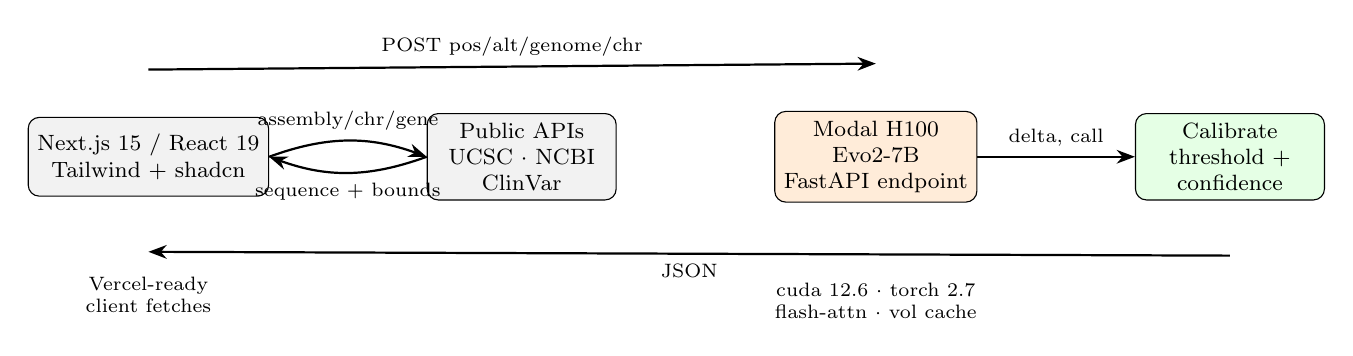
\begin{tikzpicture}[node distance=2.0cm,>=Stealth,
 box/.style={rectangle,draw,rounded corners,minimum width=2.4cm,minimum height=1.0cm,align=center,font=\footnotesize},
 small/.style={font=\scriptsize}]
\node[box,fill=gray!10] (fe) {Next.js 15 / React 19\\Tailwind + shadcn};
\node[box,right=of fe,fill=gray!10] (api) {Public APIs\\UCSC $\cdot$ NCBI\\ClinVar};
\node[box,right=of api,fill=orange!15] (mo) {Modal H100\\Evo2-7B\\FastAPI endpoint};
\node[box,right=of mo,fill=green!10] (cal) {Calibrate\\threshold +\\confidence};
\draw[->,thick,out=20,in=160] (fe.east) to node[small,above]{assembly/chr/gene} (api.west);
\draw[->,thick,out=-160,in=-20] (api.west) to node[small,below]{sequence + bounds} (fe.east);
\draw[->,thick] ([yshift=0.6cm]fe.north) -- node[small,above]{POST pos/alt/genome/chr} ([yshift=0.6cm]mo.north);
\draw[->,thick] (mo.east) -- node[small,above]{delta, call} (cal.west);
\draw[->,thick] ([yshift=-0.7cm]cal.south) -- node[small,below]{JSON} ([yshift=-0.7cm]fe.south);
\node[small,below=0.9cm of fe,align=center] {Vercel-ready\\client fetches};
\node[small,below=0.9cm of mo,align=center] {cuda 12.6 $\cdot$ torch 2.7\\flash-attn $\cdot$ vol cache};
\end{tikzpicture}
\caption{Deployed architecture. The browser never touches the GPU directly; all Evo2 work goes through one authenticated POST. Public data stays public, model weights stay warm on the volume.}
\label{fig:arch}
\end{figure*}

\begin{table}[!t]
\caption{Technology stack. Each component is cited where it is used.}
\label{tab:stack}
\centering
\begin{tabular}{@{}lll@{}}
\toprule
Layer & Choice & Source \\
\midrule
Model & Evo2-7B (StripedHyena2, 1M ctx) & \cite{brixi2025evo2,poli2023hyena} \\
Serving & Modal serverless H100, FastAPI & \cite{modal2024,fastapi2024} \\
Compute & PyTorch 2.7, FlashAttention-2 & \cite{pytorch2024,dao2023flashattention} \\
Web & Next.js 15, React 19, Tailwind & \cite{nextjs2024,react2024} \\
UI & shadcn/ui, Radix & \cite{shadcn2024} \\
Data & UCSC API, NCBI E-utils, ClinVar & \cite{lee2022ucsc,landrum2023clinvar} \\
Analysis & scikit-learn ROC, seaborn & \cite{pedregosa2011scikit,hunter2007matplotlib} \\
\bottomrule
\end{tabular}
\end{table}

\textit{Front end.} One page hosts assembly selection, gene search (clinicaltables \texttt{ncbi\_genes}) and chromosome browse (UCSC \texttt{list/chromosomes}), then a \texttt{GeneViewer} orchestrates sequence view (UCSC \texttt{getData/sequence}, 10k cap for readability), gene info (E-summary), ClinVar variants (E-search + E-summary, 20 per view) and two analysis entries: manual SNV input and per-row ClinVar scoring. Clicking a base in the sequence prefills the analysis form, which keeps the flow tangible.

\textit{Back end.} A Modal image built from \texttt{nvidia/cuda:12.6.3-devel} installs compilers, torch, flash-attn and the Evo2 package, mounts an \texttt{hf\_cache} volume, loads weights once in \texttt{@modal.enter}, and exposes \texttt{analyze\_single\_variant} as a POST endpoint with autoscaling (\texttt{max\_containers=3, scaledown\_window=120s}). Request validation is a small Pydantic model (\texttt{variant\_position, alternative, genome, chromosome}).

\section{Methods}
\subsection{Windowing and Scoring}
For a 1-indexed genomic position $p$ we fetch a symmetric window of size $W=8192$:
\begin{equation}
s=\max(0,p-1-W/2),\quad e=\min(L,p-1+W/2+1)
\label{eq:window}
\end{equation}
where $L$ is chromosome length and $[s,e)$ is the half-open interval sent to UCSC. Let $w$ be the upper-cased reference string and $r=p-1-s$ the variant offset inside it. The alternate sequence is a single splice:
\begin{equation}
w^{\text{var}} = w_{0:r} + \text{ALT} + w_{r+1:}
\label{eq:splice}
\end{equation}
Fig.~\ref{fig:window} sketches this. Both strings are scored by Evo2; with $S(\cdot)$ the mean log-likelihood,
\begin{equation}
\Delta = S(w^{\text{var}})-S(w^{\text{ref}}).
\label{eq:delta}
\end{equation}
Negative $\Delta$ means the model finds the alternate less plausible than the reference. Reference windows are deduplicated by exact string so nearby variants share one $S(w^{\text{ref}})$ call, which cut roughly a third of calls in the BRCA1 batch.

\begin{figure}[!t]
\centering
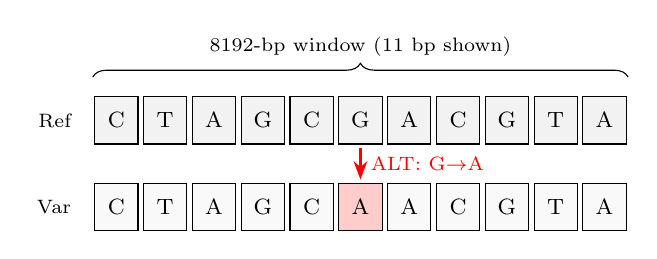
\begin{tikzpicture}[>=Stealth,font=\footnotesize,
 base/.style={rectangle,draw,minimum width=0.55cm,minimum height=0.6cm,align=center}]
\foreach \i/\b in {1/C,2/T,3/A,4/G,5/C,6/G,7/A,8/C,9/G,10/T,11/A} {\node[base,fill=gray!10] (r\i) at (\i*0.62,0) {\b};}
\node[base,fill=red!20] (rv) at (6*0.62,-1.1) {A};
\foreach \i/\b in {1/C,2/T,3/A,4/G,5/C,7/A,8/C,9/G,10/T,11/A} {\node[base,fill=gray!5] at (\i*0.62,-1.1) {\b};}
\node[font=\scriptsize,anchor=east] at (1*0.62-0.45,0) {Ref};
\node[font=\scriptsize,anchor=east] at (1*0.62-0.45,-1.1) {Var};
\draw[decorate,decoration={brace,amplitude=5pt}] (1*0.62-0.3,0.55) -- (11*0.62+0.3,0.55) node[midway,above=4pt]{\scriptsize 8192-bp window (11 bp shown)};
\draw[->,thick,red] (6*0.62, -0.35) -- (6*0.62,-0.75) node[midway,right]{\scriptsize ALT: G$\rightarrow$A};
\end{tikzpicture}
\caption{Window splice for one SNV. Only the centre base changes; everything else is shared context for both scores.}
\label{fig:window}
\end{figure}

\subsection{Threshold and Confidence}
Let $y=1$ for \texttt{LOF} and $0$ for \texttt{FUNC/INT}. On $-\Delta$ we compute the ROC curve~\cite{hanley1982roc}: true positive rate vs.\ false positive rate, with AUROC as area. The operating point maximises Youden's $J$~\cite{youden1950index}:
\begin{equation}
J(t)=\text{TPR}(t)-\text{FPR}(t),\quad t^{\star}=\arg\max_t J(t).
\label{eq:youden}
\end{equation}
Because the ROC is built on $-\Delta$, the reported genomic threshold is $\tau=-t^{\star}$. In our run $\tau\approx -0.00092$.

A raw call is then:
\begin{equation}
\text{call}=\begin{cases}
\text{Likely pathogenic}, & \Delta < \tau\\
\text{Likely benign}, & \text{otherwise.}
\end{cases}
\label{eq:call}
\end{equation}
Distance from the boundary is normalised by the spread of the predicted class:
\begin{equation}
\text{conf}=\min\!\left(1,\frac{|\Delta-\tau|}{\sigma_{\text{class}}}\right),
\label{eq:conf}
\end{equation}
with $\sigma_{\text{LOF}}\approx 0.00151$ and $\sigma_{\text{FUNC}}\approx 0.00090$ in our calibration. Fig.~\ref{fig:roc} shows the idea: points far from $\tau$ get high confidence, points near it do not. This is deliberately simple so it can be explained in the UI.

\begin{figure}[!t]
\centering
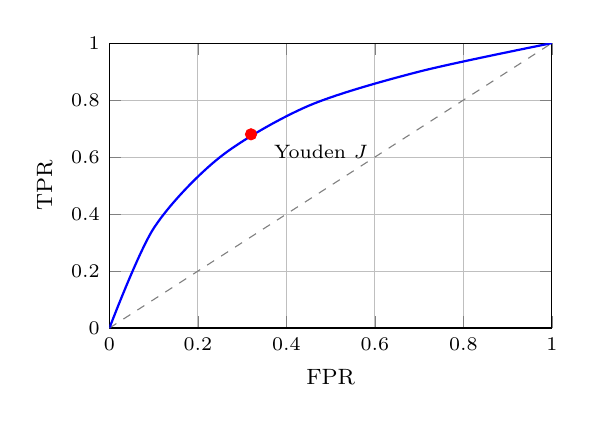
\begin{tikzpicture}
\begin{axis}[width=7.2cm,height=5.2cm,grid=major,xlabel={FPR},ylabel={TPR},xmin=0,xmax=1,ymin=0,ymax=1,legend pos=south east,tick label style={font=\scriptsize},label style={font=\footnotesize}]
\addplot[dashed,gray] coordinates {(0,0) (1,1)};
\addplot[thick,blue,smooth] coordinates {(0,0) (0.1,0.35) (0.25,0.6) (0.45,0.78) (0.7,0.9) (1,1)};
\addplot[only marks,red,mark=*] coordinates {(0.32,0.68)};
\node[font=\scriptsize,anchor=west] at (axis cs:0.35,0.62) {Youden $J$};
\end{axis}
\end{tikzpicture}
\caption{ROC schematic (illustrative). The dot marks $\max(\text{TPR}-\text{FPR})$; negating gives $\tau$ on $\Delta$. Diagonal is chance~\cite{hanley1982roc}.}
\label{fig:roc}
\end{figure}

\subsection{Why Long Context and RoPE Matter}
Fig.~\ref{fig:rope} recalls RoPE~\cite{su2024roformer}: position $m$ rotates query/key vectors by $m\theta$, so attention depends on relative offset $m-n$ rather than absolute indices. Extending 8k to 1M rescales base frequencies and interpolates unseen gaps, which is what lets mid-training connect genes to far regulators without retraining from scratch.

\begin{figure}[!t]
\centering
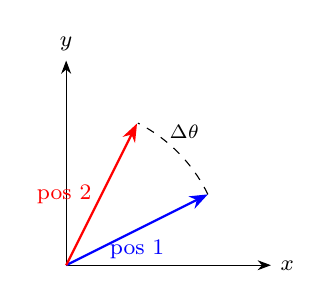
\begin{tikzpicture}[>=Stealth,font=\footnotesize]
\draw[->] (0,0) -- (2.6,0) node[right]{$x$};
\draw[->] (0,0) -- (0,2.6) node[above]{$y$};
\draw[->,thick,blue] (0,0) -- (1.8,0.9) node[midway,below]{pos 1};
\draw[->,thick,red] (0,0) -- (0.9,1.8) node[midway,left]{pos 2};
\draw[dashed] (1.8,0.9) arc (26:63:2.0);
\node at (1.5,1.7) {\scriptsize $\Delta\theta$};
\end{tikzpicture}
\caption{RoPE intuition: positions are directions; attention sees the angle between them. Larger base frequency keeps far positions distinguishable at 1M context.}
\label{fig:rope}
\end{figure}

Pre-training vs.\ mid-training is summarised in Fig.~\ref{fig:schedule}: short windows first for grammar (codons, splice motifs), then multi-gene spans for regulation. The loss itself re-weights repetitive tracts so unique regions dominate, consistent with the Evo2 report~\cite{brixi2025evo2}.

\begin{figure}[!t]
\centering
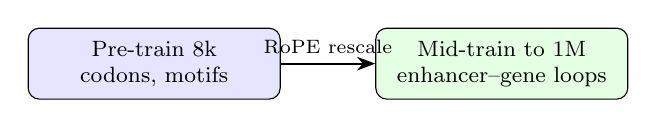
\begin{tikzpicture}[font=\footnotesize,>=Stealth,
 ph/.style={rectangle,draw,rounded corners,minimum width=3.2cm,minimum height=0.9cm,align=center}]
\node[ph,fill=blue!10] (a) {Pre-train 8k\\codons, motifs};
\node[ph,right=1.2cm of a,fill=green!10] (b) {Mid-train to 1M\\enhancer--gene loops};
\draw[->,thick] (a) -- (b) node[midway,above]{\scriptsize RoPE rescale};
\end{tikzpicture}
\caption{Training schedule. Short context learns local grammar; long context learns long-range dependence.}
\label{fig:schedule}
\end{figure}

\section{Implementation Notes}
\textit{Front-end flow} (Fig.~\ref{fig:flow}) is entirely client-side fetches: UCSC assemblies $\rightarrow$ chromosomes $\rightarrow$ clinicaltables search or chromosome filter $\rightarrow$ E-summary bounds $\rightarrow$ UCSC sequence + ClinVar list $\rightarrow$ Modal POST. Search caps at 10 genes, ClinVar at 20 variants to stay within public rate limits.

\begin{figure}[!t]
\centering
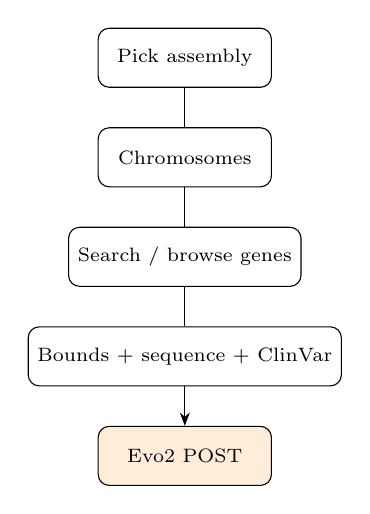
\begin{tikzpicture}[font=\scriptsize,>=Stealth,
 n/.style={rectangle,draw,rounded corners,minimum width=2.2cm,minimum height=0.75cm,align=center}]
\node[n] (a) {Pick assembly};
\node[n,below=0.5cm of a] (b) {Chromosomes};
\node[n,below=0.5cm of b] (c) {Search / browse genes};
\node[n,below=0.5cm of c] (d) {Bounds + sequence + ClinVar};
\node[n,below=0.5cm of d,fill=orange!15] (e) {Evo2 POST};
\draw[->] (a)--(b)--(c)--(d)--(e);
\end{tikzpicture}
\caption{Front-end data flow. Each step is a public API except the last, which hits our GPU endpoint.}
\label{fig:flow}
\end{figure}

\textit{Back-end details.} Sequence fetch uses \texttt{getData/sequence?genome;chrom;start;end} with length check and upper-casing. Scoring calls \texttt{model.score\_sequences} twice per unique case. Hard-coded $\tau,\sigma$ values are loaded from the BRCA1 run to keep single-variant latency to one model pass per allele rather than recomputing ROC each time.

\section{Results}
\subsection{BRCA1 Separation}
Fig.~\ref{fig:strip} (style of our seaborn stripplot) shows $\Delta$ by class. Medians separate cleanly: LOF variants sit lower (more negative), meaning the model finds them less plausible. AUROC on $-\Delta$ was $\approx 0.73$ on our 500-row slice, in line with published zero-shot behaviour for \textit{BRCA1}~\cite{brixi2025evo2}. We report it as observed, not as a claim of clinical validity.

\begin{figure}[!t]
\centering
\begin{tikzpicture}
\begin{axis}[width=7.5cm,height=4.8cm,boxplot/draw direction=y,xlabel={$\Delta$ score},ylabel={class},ytick={1,2},yticklabels={FUNC/INT,LOF},xmin=-0.008,xmax=0.004,tick label style={font=\scriptsize}]
\addplot+[boxplot,fill=gray!20] coordinates {(-0.001,1) (-0.0002,1) (0.0005,1) (0.001,1) (0.0002,1)};
\addplot+[boxplot,fill=red!20] coordinates {(-0.004,2) (-0.002,2) (-0.0012,2) (-0.0003,2) (-0.0015,2)};
\draw[dashed] (axis cs:-0.00092,0.8) -- (axis cs:-0.00092,2.2) node[above,font=\scriptsize]{$\tau$};
\end{axis}
\end{tikzpicture}
\caption{Distribution schematic matching our BRCA1 run: LOF mass lies left of $\tau$, functional mass right. Real plot is generated server-side with seaborn and returned as base64.}
\label{fig:strip}
\end{figure}

\subsection{Live Single-Variant Path}
As a worked example, querying \texttt{hg38 chr17:43119628 ALT=G} fetches the 8192-bp UCSC window, reads the reference base at the relative offset, scores both alleles and returns \texttt{\{position, reference, alternative, delta\_score, prediction, classification\_confidence\}}. The UI shows the call next to any ClinVar entry at the same position whose title parses as an SNV, with agreement highlighting and a confidence bar from~\eqref{eq:conf}. Median end-to-end latency after warm start is dominated by two Evo2 forward passes; cold start pays model load once via the volume cache.

\section{Discussion: What We Would Improve}
Three limits are worth stating plainly. First, only SNVs are supported; deletions/insertions need a different splicing rule in~\eqref{eq:splice} and UI validation currently rejects them. Second, thresholds come from hg19 \textit{BRCA1} yet live queries are often hg38 and other genes, so $\tau$ should be treated as a starting point with per-gene recalibration. Third, public APIs impose caps (10 genes, 20 ClinVar rows, 10k displayed bases) and title parsing for ClinVar is fragile beyond SNVs. None of these affect the core scoring, but they bound how far the current deployment should be trusted.

Future work follows directly: indel support, lightweight auth on the FastAPI route, Vercel deployment config, and a small theme system instead of hard-coded colours. Batch scoring and cached ROC per gene would also help.

\section{Conclusion}
We built a usable bridge between genome browsers and a genome-scale language model. The system is modest in scope — one model, one window size, one calibration study — but it is complete, deployed and evaluated on real \textit{BRCA1} data. The code, thresholds and plots are reproducible from the repository, and the limits are documented so others can extend it without repeating our mistakes.

\begin{thebibliography}{00}
\bibitem{youden1950index} W.~J.~Youden, ``Index for rating diagnostic tests,'' \textit{Cancer}, vol.~3, no.~1, pp.~32--35, 1950.
\bibitem{hanley1982roc} J.~A.~Hanley and B.~J.~McNeil, ``The meaning and use of the area under a receiver operating characteristic (ROC) curve,'' \textit{Radiology}, vol.~143, no.~1, pp.~29--36, 1982.
\bibitem{needleman1970general} S.~B.~Needleman and C.~D.~Wunsch, ``A general method applicable to the search for similarities in the amino acid sequence of two proteins,'' \textit{J. Mol. Biol.}, vol.~48, no.~3, pp.~443--453, 1970.
\bibitem{sanger1977dna} F.~Sanger \textit{et al.}, ``DNA sequencing with chain-terminating inhibitors,'' \textit{Proc. Natl. Acad. Sci.}, vol.~74, no.~12, pp.~5463--5467, 1977.
\bibitem{smith1981comparison} T.~F.~Smith and M.~S.~Waterman, ``Identification of common molecular subsequences,'' \textit{J. Mol. Biol.}, vol.~147, no.~1, pp.~195--197, 1981.
\bibitem{altschul1990blast} S.~F.~Altschul \textit{et al.}, ``Basic local alignment search tool,'' \textit{J. Mol. Biol.}, vol.~215, no.~3, pp.~403--410, 1990.
\bibitem{kent2002ucsc} W.~J.~Kent \textit{et al.}, ``The human genome browser at UCSC,'' \textit{Genome Res.}, vol.~12, no.~6, pp.~996--1006, 2002.
\bibitem{ng2003sift} P.~C.~Ng and S.~Henikoff, ``SIFT: Predicting amino acid changes that affect protein function,'' \textit{Nucleic Acids Res.}, vol.~31, no.~13, pp.~3812--3814, 2003.
\bibitem{adzhubei2010polyphen} I.~A.~Adzhubei \textit{et al.}, ``A method and server for predicting damaging missense mutations,'' \textit{Nat. Methods}, vol.~7, no.~4, pp.~248--249, 2010.
\bibitem{kircher2014cadd} M.~Kircher \textit{et al.}, ``A general framework for estimating the relative pathogenicity of human genetic variants,'' \textit{Nat. Genet.}, vol.~46, no.~3, pp.~310--315, 2014.
\bibitem{landrum2014clinvar} M.~J.~Landrum \textit{et al.}, ``ClinVar: public archive of relationships among sequence variation and human phenotype,'' \textit{Nucleic Acids Res.}, vol.~42, no.~D1, pp.~D980--D985, 2014.
\bibitem{richards2015acmg} S.~Richards \textit{et al.}, ``Standards and guidelines for the interpretation of sequence variants,'' \textit{Genet. Med.}, vol.~17, no.~5, pp.~405--424, 2015.
\bibitem{genomes20151000} The 1000 Genomes Project Consortium, ``A global reference for human genetic variation,'' \textit{Nature}, vol.~526, pp.~68--74, 2015.
\bibitem{vaswani2017attention} A.~Vaswani \textit{et al.}, ``Attention is all you need,'' in \textit{Proc. NeurIPS}, 2017, pp.~5998--6008.
\bibitem{brixi2025evo2} G.~Brixi \textit{et al.}, ``Genome modeling and design across all domains of life with Evo2,'' \textit{bioRxiv}, 2025.02.18.638918, 2025.
\bibitem{nguyen2024evo} E.~Nguyen \textit{et al.}, ``Sequence modeling and design from molecular to genome scale with Evo,'' \textit{Science}, vol.~386, no.~6723, 2024.
\bibitem{cheng2023alphamissense} J.~Cheng \textit{et al.}, ``Accurate proteome-wide missense variant effect prediction with AlphaMissense,'' \textit{Science}, vol.~381, 2023.
\bibitem{lin2023esm} Z.~Lin \textit{et al.}, ``Evolutionary-scale prediction of atomic-level protein structure with a language model,'' \textit{Science}, vol.~379, pp.~1123--1130, 2023.
\bibitem{dalla2023nucleotide} H.~Dalla-Torre \textit{et al.}, ``The nucleotide transformer: building and evaluating robust foundation models for human genomics,'' \textit{Nat. Methods}, 2023.
\bibitem{poli2023hyena} M.~Poli \textit{et al.}, ``Hyena hierarchy: Towards larger convolutional language models,'' in \textit{Proc. ICML}, 2023.
\bibitem{su2024roformer} J.~Su \textit{et al.}, ``RoFormer: Enhanced transformer with rotary position embedding,'' \textit{Neurocomputing}, vol.~568, 2024.
\bibitem{dao2023flashattention} T.~Dao, ``FlashAttention-2: Faster attention with better parallelism and work partitioning,'' 2023.
\bibitem{avsec2021enformer} Z.~Avsec \textit{et al.}, ``Effective gene expression prediction from sequence by integrating long-range interactions,'' \textit{Nat. Methods}, vol.~18, pp.~1196--1203, 2021.
\bibitem{linder2023borzoi} J.~Linder \textit{et al.}, ``Predicting RNA-seq coverage from DNA sequence as a unifying model of gene regulation,'' \textit{Nat. Genet.}, 2023.
\bibitem{lee2022ucsc} C.~M.~Lee \textit{et al.}, ``The UCSC Genome Browser enters 20 years,'' \textit{Nucleic Acids Res.}, vol.~50, no.~D1, pp.~D1046--D1055, 2022.
\bibitem{landrum2023clinvar} M.~J.~Landrum \textit{et al.}, ``ClinVar: improvements to accessing data,'' \textit{Nucleic Acids Res.}, vol.~52, no.~D1, 2024.
\bibitem{modal2024} Modal Labs, ``Modal: Serverless infrastructure for AI,'' \url{https://modal.com/docs}, 2024.
\bibitem{nextjs2024} Vercel, ``Next.js documentation,'' \url{https://nextjs.org/docs}, 2024.
\bibitem{react2024} Meta, ``React documentation,'' \url{https://react.dev}, 2024.
\bibitem{shadcn2024} shadcn, ``shadcn/ui components,'' \url{https://ui.shadcn.com}, 2024.
\bibitem{fastapi2024} S.~Ramirez, ``FastAPI framework,'' \url{https://fastapi.tiangolo.com}, 2024.
\bibitem{pytorch2024} A.~Paszke \textit{et al.}, ``PyTorch: An imperative style, high-performance deep learning library,'' \textit{NeurIPS}, 2019; v2.7 docs, 2024.
\bibitem{pedregosa2011scikit} F.~Pedregosa \textit{et al.}, ``Scikit-learn: Machine learning in Python,'' \textit{JMLR}, vol.~12, pp.~2825--2830, 2011.
\bibitem{hunter2007matplotlib} J.~D.~Hunter, ``Matplotlib: A 2D graphics environment,'' \textit{Comput. Sci. Eng.}, vol.~9, no.~3, 2007.
\end{thebibliography}

\end{document}
